% Options for packages loaded elsewhere
\PassOptionsToPackage{unicode}{hyperref}
\PassOptionsToPackage{hyphens}{url}
\PassOptionsToPackage{dvipsnames,svgnames,x11names}{xcolor}
%
\documentclass[
  authoryear,
  preprint,
  3p]{elsarticle}

\usepackage{amsmath,amssymb}
\usepackage{lmodern}
\usepackage{iftex}
\ifPDFTeX
  \usepackage[T1]{fontenc}
  \usepackage[utf8]{inputenc}
  \usepackage{textcomp} % provide euro and other symbols
\else % if luatex or xetex
  \usepackage{unicode-math}
  \defaultfontfeatures{Scale=MatchLowercase}
  \defaultfontfeatures[\rmfamily]{Ligatures=TeX,Scale=1}
\fi
% Use upquote if available, for straight quotes in verbatim environments
\IfFileExists{upquote.sty}{\usepackage{upquote}}{}
\IfFileExists{microtype.sty}{% use microtype if available
  \usepackage[]{microtype}
  \UseMicrotypeSet[protrusion]{basicmath} % disable protrusion for tt fonts
}{}
\makeatletter
\@ifundefined{KOMAClassName}{% if non-KOMA class
  \IfFileExists{parskip.sty}{%
    \usepackage{parskip}
  }{% else
    \setlength{\parindent}{0pt}
    \setlength{\parskip}{6pt plus 2pt minus 1pt}}
}{% if KOMA class
  \KOMAoptions{parskip=half}}
\makeatother
\usepackage{xcolor}
\setlength{\emergencystretch}{3em} % prevent overfull lines
\setcounter{secnumdepth}{5}
% Make \paragraph and \subparagraph free-standing
\ifx\paragraph\undefined\else
  \let\oldparagraph\paragraph
  \renewcommand{\paragraph}[1]{\oldparagraph{#1}\mbox{}}
\fi
\ifx\subparagraph\undefined\else
  \let\oldsubparagraph\subparagraph
  \renewcommand{\subparagraph}[1]{\oldsubparagraph{#1}\mbox{}}
\fi


\providecommand{\tightlist}{%
  \setlength{\itemsep}{0pt}\setlength{\parskip}{0pt}}\usepackage{longtable,booktabs,array}
\usepackage{calc} % for calculating minipage widths
% Correct order of tables after \paragraph or \subparagraph
\usepackage{etoolbox}
\makeatletter
\patchcmd\longtable{\par}{\if@noskipsec\mbox{}\fi\par}{}{}
\makeatother
% Allow footnotes in longtable head/foot
\IfFileExists{footnotehyper.sty}{\usepackage{footnotehyper}}{\usepackage{footnote}}
\makesavenoteenv{longtable}
\usepackage{graphicx}
\makeatletter
\def\maxwidth{\ifdim\Gin@nat@width>\linewidth\linewidth\else\Gin@nat@width\fi}
\def\maxheight{\ifdim\Gin@nat@height>\textheight\textheight\else\Gin@nat@height\fi}
\makeatother
% Scale images if necessary, so that they will not overflow the page
% margins by default, and it is still possible to overwrite the defaults
% using explicit options in \includegraphics[width, height, ...]{}
\setkeys{Gin}{width=\maxwidth,height=\maxheight,keepaspectratio}
% Set default figure placement to htbp
\makeatletter
\def\fps@figure{htbp}
\makeatother

\newcommand{\yg}[1]{{\textcolor{orange}{#1}}}
\newcommand{\svp}[1]{{\textcolor{blue}{#1}}}
\newcommand{\ak}[1]{{\textcolor{purple}{#1}}}
\makeatletter
\makeatother
\makeatletter
\makeatother
\makeatletter
\@ifpackageloaded{caption}{}{\usepackage{caption}}
\AtBeginDocument{%
\ifdefined\contentsname
  \renewcommand*\contentsname{Table of contents}
\else
  \newcommand\contentsname{Table of contents}
\fi
\ifdefined\listfigurename
  \renewcommand*\listfigurename{List of Figures}
\else
  \newcommand\listfigurename{List of Figures}
\fi
\ifdefined\listtablename
  \renewcommand*\listtablename{List of Tables}
\else
  \newcommand\listtablename{List of Tables}
\fi
\ifdefined\figurename
  \renewcommand*\figurename{Figure}
\else
  \newcommand\figurename{Figure}
\fi
\ifdefined\tablename
  \renewcommand*\tablename{Table}
\else
  \newcommand\tablename{Table}
\fi
}
\@ifpackageloaded{float}{}{\usepackage{float}}
\floatstyle{ruled}
\@ifundefined{c@chapter}{\newfloat{codelisting}{h}{lop}}{\newfloat{codelisting}{h}{lop}[chapter]}
\floatname{codelisting}{Listing}
\newcommand*\listoflistings{\listof{codelisting}{List of Listings}}
\makeatother
\makeatletter
\@ifpackageloaded{caption}{}{\usepackage{caption}}
\@ifpackageloaded{subcaption}{}{\usepackage{subcaption}}
\makeatother
\makeatletter
\@ifpackageloaded{tcolorbox}{}{\usepackage[many]{tcolorbox}}
\makeatother
\makeatletter
\@ifundefined{shadecolor}{\definecolor{shadecolor}{rgb}{.97, .97, .97}}
\makeatother
\makeatletter
\makeatother
\journal{Journal Name}
\ifLuaTeX
  \usepackage{selnolig}  % disable illegal ligatures
\fi
\usepackage[]{natbib}
\bibliographystyle{elsarticle-harv}
\IfFileExists{bookmark.sty}{\usepackage{bookmark}}{\usepackage{hyperref}}
\IfFileExists{xurl.sty}{\usepackage{xurl}}{} % add URL line breaks if available
\urlstyle{same} % disable monospaced font for URLs
\hypersetup{
  pdftitle={Redesigning Yield Map Plots for Comprehension and Usability},
  pdfauthor={Alison Kleffner; Susan Vanderplas},
  pdfkeywords={visualization, spatial correlation},
  colorlinks=true,
  linkcolor={blue},
  filecolor={Maroon},
  citecolor={Blue},
  urlcolor={Blue},
  pdfcreator={LaTeX via pandoc}}

\setlength{\parindent}{6pt}
\begin{document}

\begin{frontmatter}
\title{Redesigning Yield Map Plots for Comprehension and Usability}
\author[1]{Alison Kleffner%
%
\fnref{fn1}}
 \ead{akleffner@huskers.unl.edu} 
\author[2]{Susan Vanderplas%
\corref{cor1}%
}
 \ead{susan.vanderplas@unl.edu} 

\affiliation[1]{organization={University of
Nebraska-Lincoln, Statistics},addressline={340 Hardin Hall North Wing
3310 Holdrege},city={Lincoln},postcode={68583},postcodesep={}}
\affiliation[2]{organization={},,postcodesep={}}

\cortext[cor1]{Corresponding author}
\fntext[fn1]{This is the first author footnote.}

        
\begin{abstract}
A standard method to display the relationship between two variables is
through visualization. However, if these variables occupy the same
spatial domain, there is difficulty in perceiving any statistical
relationships between the data. Data occupying the same spatial domain
is common in the agricultural field, and while visualizations in this
area exist, they do not conform to the principles of effective chart
design. As a motivating example to illustrate challenges and potential
solutions, we examined visualizing the relationship between crop input
application and crop yield. Understanding this relationship is crucial
as inefficiently applying crop inputs, like nitrogen fertilizer, impacts
profit and the environment. The purpose of the Data Intensive Farm
Management (DIFM) project is to allow farmers to run experiments that
establish the effect of crop application on yield in specific locations.
These trials, called On-Farm Precision Experiments (OFPE), leverage the
ability to precisely control the application type and rate using
GPS-enabled machinery while conducting these experiments. While maps
attempting to display this relationship exist, they do not follow the
principles of effective chart design. Our objectives are to identify the
perceptual issues in current visualizations from our motivating example
and to propose plots to mitigate these challenges. By documenting the
process of improving graphics to increase comprehension and ease of use,
these ideas can be used with similar data in the agricultural field to
display it better. Visualizing the data more effectively makes the
information presented more attainable for more people and may allow
further insight into the data.
\end{abstract}





\begin{keyword}
    visualization \sep 
    spatial correlation
\end{keyword}
\end{frontmatter}
    \ifdefined\Shaded\renewenvironment{Shaded}{\begin{tcolorbox}[interior hidden, enhanced, sharp corners, breakable, boxrule=0pt, frame hidden, borderline west={3pt}{0pt}{shadecolor}]}{\end{tcolorbox}}\fi

\hypertarget{introduction}{%
\section{Introduction}\label{introduction}}

With a projected increase in future crop demand, researchers are
conducting studies on crop input application to increase yield, focusing
on sustainability \citep{tilman_sustainalbe_2011}. The systematic
inefficient application of crop inputs on farm fields is a worldwide
issue. Examples of typical crop inputs include nitrogen fertilizer and
seeds. For instance, farmers seek to aid crop growth by introducing
nitrogen fertilizer to their fields, as under natural conditions, the
amount of nitrogen in the soil is small \citep{gruber_nitrogen_2008}.
Nitrogen is an essential component of food production as it is a
component of amino acids, the building blocks of proteins, and allows
plants to photosynthesize efficiently \citep{MAHESWARI2017175}.
Unfortunately, nearly half of the nitrogen fertilizer supplied to the
field is not used by crops, resulting in excess nitrogen in the
ecosystem \citep{billen_nitrogen_2013}. This excess nitrogen can be
harmful to the environment
\citep{NIKOLENKO20181415, menegat-nitrogen-2021}. Excess nitrogen use
may also impact profits, as farmers purchase more nitrogen than
necessary. Current adoption of tools that aid in decision-making is low.
So the focus has turned to using more data-driven decision making and
building tools to aid with this. To collect the data and build the
tools, more research needs to be conducted.

The Data Intensive Farm Management (DIFM) Project's purpose is to
develop cyber-infrastructure to easily generate the data necessary for a
better understanding of this problem by allowing farmers to run
experiments that establish the effect of crop input application on the
yield on their fields \citep{bullock-grant-2019}. This data can support
more optimal decision-making by finding an optimal application rate that
balances profit and sustainability
\citep{kyveryga-farm-2019, value-on-farm-2020}. These trials, called
On-Farm Precision Experiments (OFPE), leverage the ability to conduct an
experimental design developed using site-specific information and
precisely controlling the input application rate using GPS-enabled
agricultural machinery \citep{bullock-grant-2019}. These experiments
then help inform optimal management decisions.

To design these experiments, farmers use an open-source web-based trial
design tool developed in \emph{R Shiny}
(\href{http://trialdesign.difm-cig.org/}{link}) that allows for the
specification of plot dimension, treatment type (generally nitrogen or
seed), treatment rates, and equipment parameters, among other factors.
Then, the web-based tool creates an appropriate experimental design
(usually latin-square based) using these inputs. Once the user is
satisfied with the experimental design, the web-based tool generates
shape files that are then entered into their input machine to direct the
application of treatments at the specified rates in the designated
locations per the experimental design. After planting, the equipment
generates a shape file containing the as-applied rates (which differ
from the target rates due to sensor error and machine limits)
\citep{trevisan-spatial-2021}. At the end of the growing season,
harvesting equipment generates similar shape files containing yield
measurements and their measurement location.

While statistical and machine learning models are beneficial tools to
help determine the site-specific optimal rates, it is also valuable to
visually explore the collected data on how crop yield responds to
different input application rates at various locations on the field.
Hopefully, by visually showing this relationship, trust is built in
eventual machine learning output on optimal management decisions. A
general principle of data visualization is to show the data and to show
it clearly \citep{gordon_2015}. In this scenario, following this
principle is difficult, as the different shape files (planned,
as-applied, harvested) occupy the same spatial domain, making it
extremely difficult to visualize in a way that allows the viewer to
perceive any statistical relationship between the data. While yield maps
attempting to display the data exist, they do not conform to the
principles of effective chart design. Ineffective visualizations can
lead to longer graph comprehension time, decrease readability of a
graph, and an inability to discover or the incorrect discovery of
patterns \citep{Miller1956TheMN, macdonald_1999, huang2009, lyi2021}.

The organization of this paper is as follows:

\begin{itemize}
\tightlist
\item
  In Section 2, we analyze the shortcoming of such yield maps and
  document the map design process to maintain the spatial context of the
  data while allowing viewers to perceive relationships between
  variables. Maintaining spatial context is crucial as yield can vary
  spatially due to variables like soil variability.
\item
  Section 3 presents our process to produce useful and visually engaging
  charts for a wide variety of users (farmers, researchers, crop
  consultants) while adhering to the principles of good chart design.
\item
  The last section summarizes the main criticisms of current yield maps
  and discusses our proposed improvements.
\end{itemize}

\hypertarget{yield-maps-and-graphical-perception}{%
\section{Yield Maps and Graphical
Perception}\label{yield-maps-and-graphical-perception}}

\begin{figure}

\begin{minipage}[t]{0.50\linewidth}

{\centering 

\raisebox{-\height}{

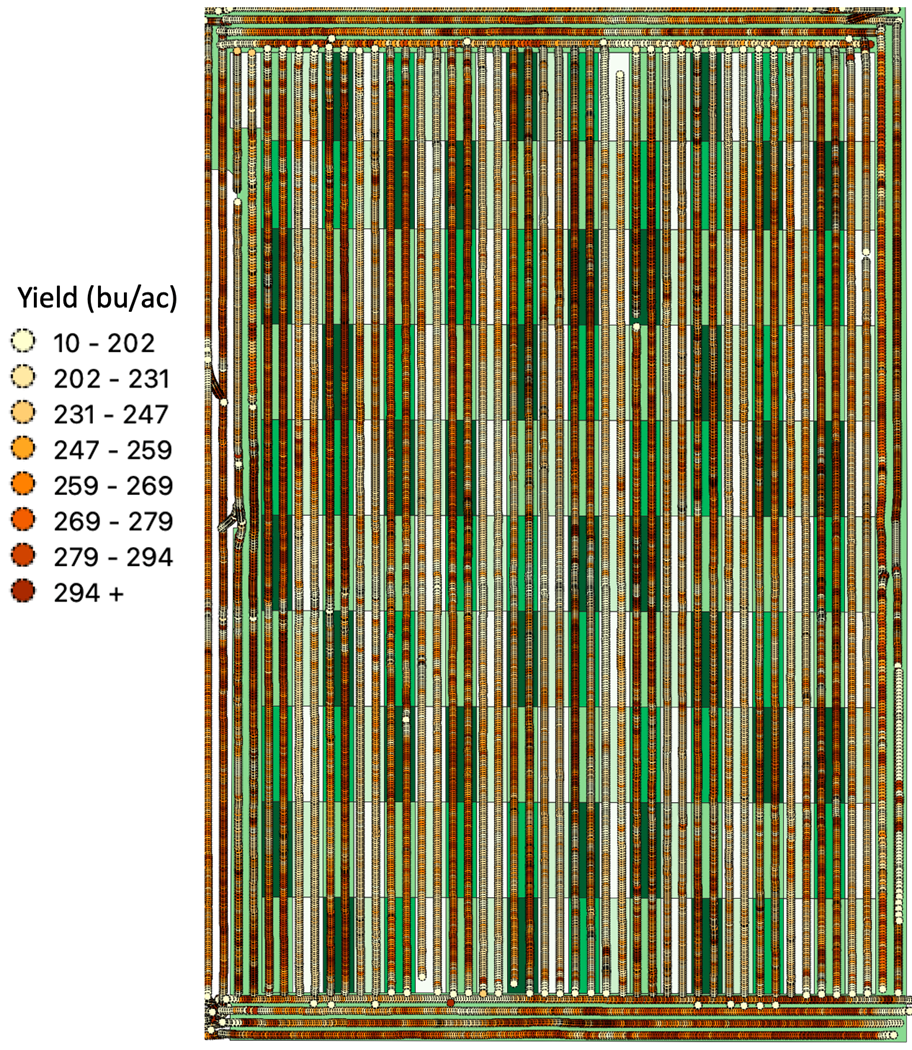
\includegraphics{../images/old_map.png}

}

}

\subcaption{\label{fig-difmmap1a}Seed Trial}
\end{minipage}%
%
\begin{minipage}[t]{0.50\linewidth}

{\centering 

\raisebox{-\height}{

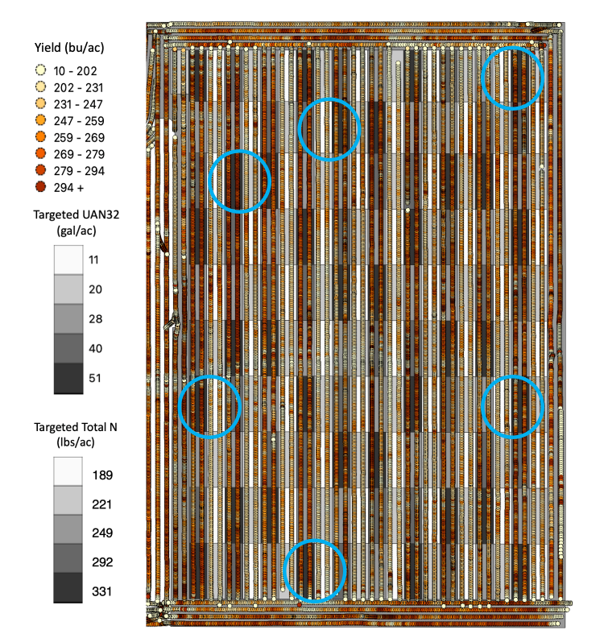
\includegraphics{../images/paper/nitrogen-trial.png}

}

}

\subcaption{\label{fig-difmmap1b}Nitrogen Trial}
\end{minipage}%

\caption{\label{fig-maps}Example of a current map produced by DIFM for
farmers that superimposes the trial design and yield information. These
figures represent a seed and nitrogen trial conducted simultaneously.
The blue circles in (b) were manually added to denote areas where the
lowest target nitrogen group and highest nitrogen group are
side-by-side. They generally show that low yield is associated with the
lowest target and high yield with the highest target rate. These plots
violate several principles of effective chart design, like failing to
show the data clearly.}

\end{figure}

Figure~\ref{fig-maps} is an example of a map given to farmers and
consultants. On this field, a seed and nitrogen trial were conducted
simultaneously, with each input trial represented on a separate map.
This figure superimposes the yield map (same for both
Figure~\ref{fig-difmmap1a} and Figure~\ref{fig-difmmap1b}) on top of the
trial design map provided by the trial design tool. The colored
rectangles (green scale for seeds and grayscale for nitrogen) represent
the underlying trial design, with the different color hues representing
the planned treatments. The overlaid yield plot is made of circles
representing the yield measurement location, as recorded by the
harvesting equipment. The circle color represents the crop yield amount
in bu/acre, which in this example represents corn yield. The plot was
developed using QGIS.

Design choices made in both plots make them perceptually sub-optimal.
First, the circles representing the harvested crop yield overlap,
obstructing the visual cue of color, thereby reducing the search
efficiency \citep{BRAVO2004b, BRAVO2004a}. Due to the overlap,
distinguishing the circle color requires more effort, made even more
difficult by its black outline. As a consequence of the color
obstruction, errors may occur when searching for a pattern between yield
and treatment, the goal of the map, as the density of the overlapping
measurement burdens the human perception \citep{huang2009}. Clutter
issues are common among superimposed graphics, as these graphs attempt
to display multiple variables in the same space \citep{gleicher2011}.\\
A second perceptual concern with Figure~\ref{fig-maps} is related to the
number of categories used to group the yield measurements (eight). Due
to working memory limits, the recommendation for categorical scales is
five to seven \citep{Miller1956TheMN, SILVA2011320}. As the number of
categories increases, it becomes harder for the user to distinguish
between colors, and remember the meaning of each color
\citep{macdonald_1999}. Hence, with more than the recommended number of
categories, it is more difficult to associate a color with the correct
yield category. The additional load on the user's cognitive system
increases the comprehension time of the graph \citep{huang2009}.
Additionally, Figure~\ref{fig-difmmap1a} omits the legend for the trial
design, so the user does not know what the target applications are and
would have to look elsewhere for this information. Transfer errors are a
drawback of making a chart in a different application (QGIS) than the
rest of the report (Word).

Finally, the chosen color scheme is another significant perceptual
concern related to the map. The use of a green gradient for the seed
trial with a red-orange gradient for yield is of particular concern.
Red-green color blindness is experienced by approximately 8\% of men and
0.5\% of women of Northern European ancestry. It is difficult for those
affected individuals to discriminate between these colors, including
colors that contain a component of those colors \citep{wong2011color}.
Thus, separating the target application rate and yield measurement would
be difficult for those users. The inability to discriminate colors
negatively impacts performance in decoding information from the plot
\citep{SILVA2011320}. Choosing the colors representing the different
variables in Figure~\ref{fig-difmmap1a} more strategically may make the
graph more accessible to this population of users.

Figure~\ref{fig-jux-plot} is another variation of this map used in DIFM
reports produced with \emph{R}. This figure only presents a nitrogen
trial. It uses juxtaposed maps, meaning the yield and trial design maps
are laid-out side by side. The trial design map is on the left side and
is identical to the underlying map in Figure~\ref{fig-difmmap1b}. On the
right side is the yield plot, where the yield point measurements were
transformed into polygons based on the distance between points, swath
width (repetitively cut strips), and headings (harvester direction).
This graph also has perceptual issues, including, once again, the choice
of the color scheme of the green and red-orange gradient. Additionally,
the color scheme for nitrogen between Figure~\ref{fig-difmmap1a} and
Figure~\ref{fig-jux-plot} is inconsistent and should be represented
uniformly in DIFM reports to lessen confusion.

Due to the juxtaposition of the two maps, Figure~\ref{fig-jux-plot} does
not have issues with visual clutter or overlapping information.
Particularly as non-overlapping polygons now represent the yield
measurements. Additionally, juxtaposed plots tend to be easier to create
than superimposed graphs. On the other hand, a juxtaposed layout places
most of the comparative burden on the users' memory
\citep{gleicher2011}. A mental image is relied on for comparison in
these scenarios, as the user moves their eyes between images (shifting
focus). The plot contents may not be accurately formed in working
memory, leading to potential errors when deriving patterns
\citep{vanderplas2020, lyi2021}. For example, the user would have to
identify the corresponding regions of each plot and then visually derive
some correlation assessment. This is a demanding set of visual and
cognitive operations, made even more difficult by the lack of visual
cues for locations.

\begin{figure}

{\centering 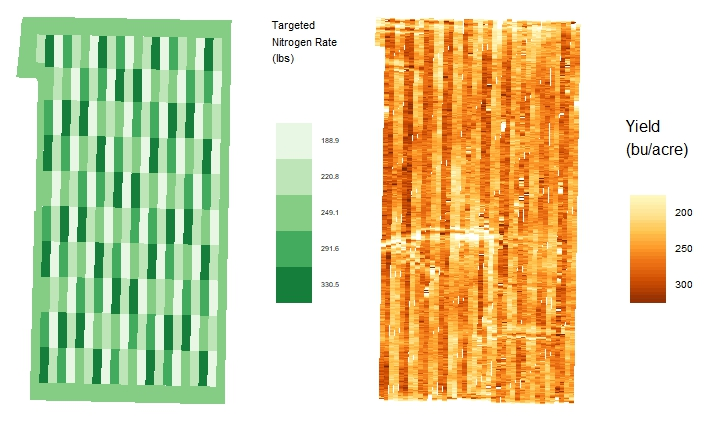
\includegraphics{../images/juxtaposed-ex.jpeg}

}

\caption{\label{fig-jux-plot}Another example of a DIFM plot, where now
the information about input application and yield for a nitrogen trial
is juxtaposed. This map poses issues as the comparative burden relies
solely on the user.}

\end{figure}

The presentation of other plots found in journals and extension
publications, likewise displaying the relationship between target
application and yield, also have perceptually sup-optimal design
choices. These examples show the widespread problem of perceptually
optimal plots in the agricultural domain. For example, a juxtaposed
layout, comprised of a target map and the distribution of yield
measurement locations, can be found in Figure 4 of
\citet{Peerlinck2018UsingDL}. The yield map is similar to
Figure~\ref{fig-maps}, due to overlapping points with a black outline.
The true number of points is then obscured, concealing information about
the yield point distribution. Users with red-green color blindness will
have difficulty accurately reading the target values on the prescription
map due to the chosen red-green color scheme. Also, the author used a
similar color scheme to represent a target value and yield points. The
overlap in color schemes is an issue as it may interfere with each when
trying to derive information. A similar situation arises in Figure 1 and
Figure 2 by \citet{poursina-nitrogen-2021}, with the same color scheme
applied to the target and yield map.

The right-hand side of Figure 4 in \citet{gardner-ag-2021} is another
example, where a slight overlap in the color scheme for the nitrogen
treatment map and yield map occurs. In addition, due to the
juxtaposition of three different plots for this field (seed rate,
nitrogen rate, yield), simultaneously comparing the maps is difficult
since high mental effort is required. The minimal spatial cues to aid in
comparing the variables across plots add to the difficulty. Figure 3 of
\citet{trevisan-spatial-2021} has similar problems. The right-hand side
of Figure 2 in \citet{maxwell-farm-2018} does use a different color
scheme for the treatment and yield map. However, the treatment variable
uses the popular but problematic rainbow color scheme. Firstly, the
rainbow color scheme is sub-optimal due to no inherent ordering of
magnitude when the input application it represents has an ordering of
magnitude \citep{light-rainbow-2004}. Secondly, the extremes are
visually close (red and violet), confusing users to differentiate values
on both ends of the scale \citep{SILVA2011320}.

Even if only displaying a yield map, the yield maps tend to have
sub-optimal design choices. Most of these choices are related to color
schemes. For example, Figure 1 in \citet{tao_ag_2019} uses a stop-light
color scheme. However, for diverging color schemes, the transition
between the two extreme colors should go through a neutral color, like
white \citep{MIDWAY2020100141}. Yellow is sub-optimal as a transition
color as it tends to have a highlighting effect \citep{SILVA2011320}.
More importantly, since the map only displays the magnitude of yield, a
univariate color scheme would be more effective \citep{vanderplas2020}.
The stop-light color scheme also would make it difficult for those who
are red-green color blind to differentiate yield values.

Another example can be found in Figure 1 from \citet{map_2020}. In this
figure, the yield measurements are obscured, concealing their true
value. Additionally, in Figure 7 in \citet{searcy1997precision}, a plot
is used to display corn yield on a farm field in Texas. This plot first
has more than the recommended number of categories (ten in total). The
squares representing each yield measurement also overlap, obstructing
the visual cue of color. Finally, a better color scheme should be
chosen, as the current color scheme does not necessarily imply an
ordering among the categories. Hence, a sequential scale of one color
from light to dark would be more appropriate and color-blind friendly
\citep{MIDWAY2020100141}. Thus, prescription and yield maps tend to have
some commonalities among their sub-optimal design choices. These include
visual clutter, the number of scale categories for yield, and color
scheme choice. We want to develop a new map that presents the same
information while also addressing the weaknesses of the previous maps.

\hypertarget{redesign}{%
\section{Redesign}\label{redesign}}

The primary purpose of this project is to document the development
process of improved alternatives to spatial correlation displays used in
agricultural applications. There are many papers on statistical
graphics, but relatively few document the improvement process to
increase comprehension, ease of use, and perceptual accuracy. First, we
considered each comparative graphic layout: superposition,
juxtaposition, and explicit encoding \citep{gleicher2011}. We decided to
start with superposition (spatial overlay) shown in
Figure~\ref{fig-maps}, as juxtaposed maps require a higher cognitive
load to compare across plots, and explicitly encoded maps do not
directly show the data \citep{lyi2021}. On the other hand, superimposed
graphs show the data while allowing the user to use their perceptual
system instead of their memory \citep{gleicher2011}. When spatial
location is a key component of the comparison, the superimposed layout
is beneficial, as the individual maps occupy the same axes
\citep{Wood2007InteractiveVE, wang_comp18}. In this section, we plan to
address the perceptual issues one at a time. We begin by addressing one
of the major issues with the original map (Figure~\ref{fig-difmmap1a}):
the overplotted circles, which make it impossible to see the yield
information, as the circle boundaries (which are not colored) are more
prominent than the shaded interior and tend to overlap.

\begin{figure}

{\centering 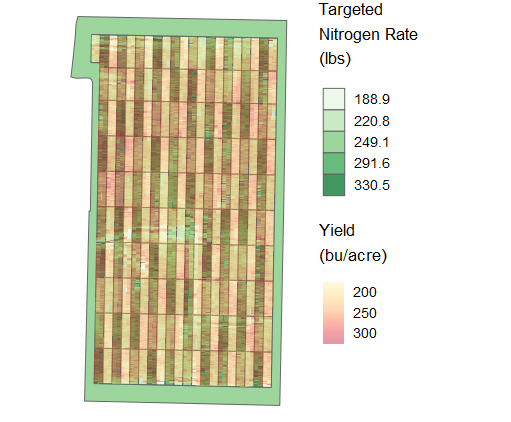
\includegraphics{../images/paper/Attempt1.png}

}

\caption{\label{fig-redesign1}The first step in the redesign process,
maintains the initial color scheme, but transparency was introduced to
allow both layers to be shown simultaneously. This potentially allows
the user to derive a correlation between these variables through
implicit color blending.}

\end{figure}

The first redesign iteration (Figure~\ref{fig-redesign1}) superimposes
the yield and trial design maps. Note that yield measurements in the
headland (the region around the trial design) are omitted, as this data
is less reliable due to differences in sun exposure and changes in
driving speed, among others. Instead of a single point for yield, we
used yield polygons to represent the area where the measurement was
taken to reduce the amount of information obscured. The yield polygons
are created in the same fashion as the yield map (right) in
Figure~\ref{fig-jux-plot}. During this first design iteration, we
maintained the (problematic) color scheme of the original to provide
continuity and obtain buy-in from domain experts who associate specific
colors with specific variables. The top layer (yield map) introduces
transparency to discern both design elements, and the relationship
between the variables is determined through blending colors
\citep{MIDWAY2020100141}. Finally, a continuous scale was used for yield
measurements instead of a discrete.

\begin{figure}

{\centering 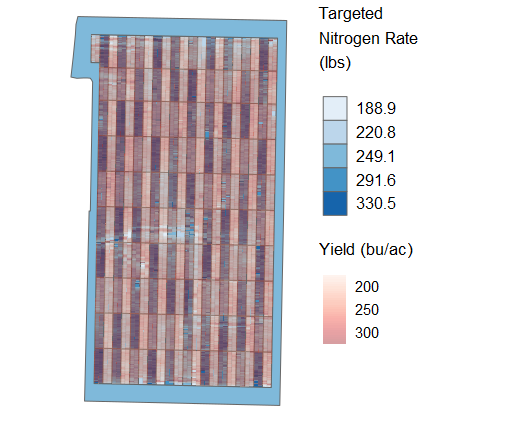
\includegraphics{../images/paper/Attempt2.png}

}

\caption{\label{fig-redesign2}The second step in the redesign process
focuses on color choice. Here, instead of the problematic red-green
color scheme, a blue sequential palette is introduced for the treatment
variables, so the two variables are distinguishable to those who are
red-green color blind.}

\end{figure}

We introduced a different color scheme in the second design iteration
(Figure~\ref{fig-redesign2}) to address the colorblindness issues from
the first iteration. We continued to use red for the response variable
(yield). In this iteration, we utilized a continuous scale for the yield
measurement. However, we chose to use a sequential blue color palette to
represent the target treatments. We chose a sequential blue scale as
\citet{wong2011color} listed it as a color that can be differentiated by
those with red-green colorblindness. Once again, we introduced
transparency for the yield variable in an attempt to blend the colors.
This map allows the user to see that higher nitrogen rates are
associated with a higher yield.

\begin{figure}

\begin{minipage}[t]{0.65\linewidth}

{\centering 

\raisebox{-\height}{

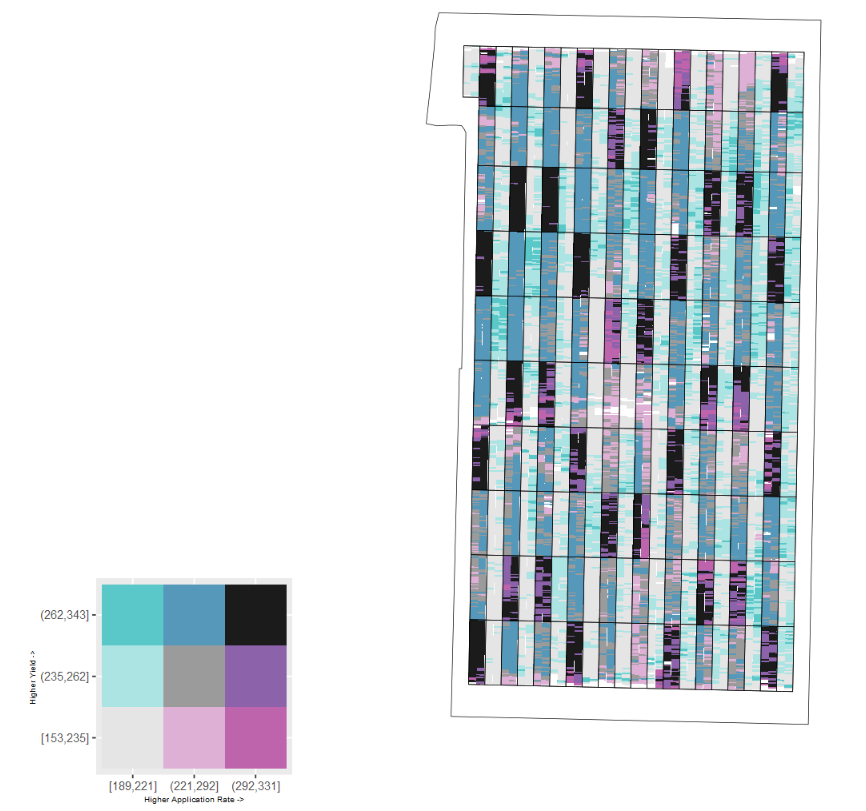
\includegraphics{../images/paper/color-map4.png}

}

}

\subcaption{\label{fig-biv-map}Bivariate Color Map}
\end{minipage}%
%
\begin{minipage}[t]{0.35\linewidth}

{\centering 

\raisebox{-\height}{

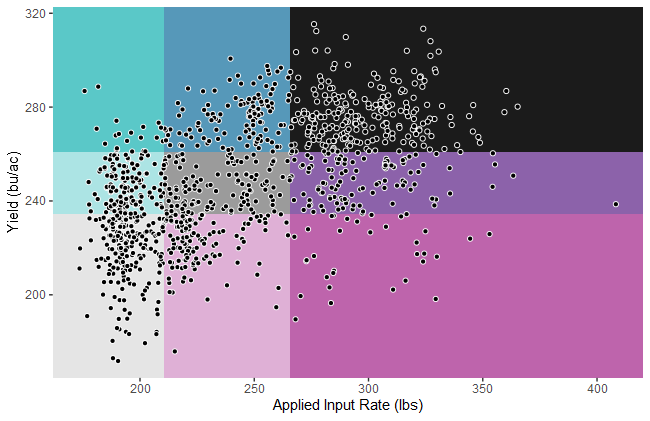
\includegraphics{../images/paper/scatt-color6.png}

}

}

\subcaption{\label{fig-biv-scat}Scatterplot of data using the same
colors}
\end{minipage}%

\caption{\label{fig-biv-color}The bivariate color map has been suggested
as an alternative to blending colors for bivariate data. In this map,
each of the variables are made into three categories. Extra attention is
focused on the diagonal of the color scheme to show the relationship
between the variables. For example, the black representing high input
application and high yield sticks out. A scatterplot is added to give
more specific information about the value of the different data points.}

\end{figure}

A bivariate color map is an alternative to color blending in displaying
the relationship between the target and yield variables. These maps can
be helpful if the relationship between the variables is more important
than the individual values \citep{elmer2013symbol}. In bivariate color
maps, two univariate color scales combine into a sequential color
scheme. A 3x3 map (3 categories for each variable) is the
recommendation, as more categories hinder interpretation
\citep{Leonowicz2003RESEARCHOT}. We chose quantiles to split the data
into low, medium, and high categories \citep{biesecker-2020}. Since we
are interested in the direct relationship between our variables, the
focus is on the diagonal, so the diagonal values used a grayscale color
scheme. Then the colors in the upper left and lower right have a
complementary color scheme to show their separation \citep{strode-2020}.
Figure~\ref{fig-biv-map} is an example of our proposed bivariate color
map. It is then easy to juxtapose this plot with a scatterplot
(Figure~\ref{fig-biv-scat}). In this plot, the points represent the
as-applied versus the yield, colored by the category from the bivariate
color map.

\begin{figure}

{\centering 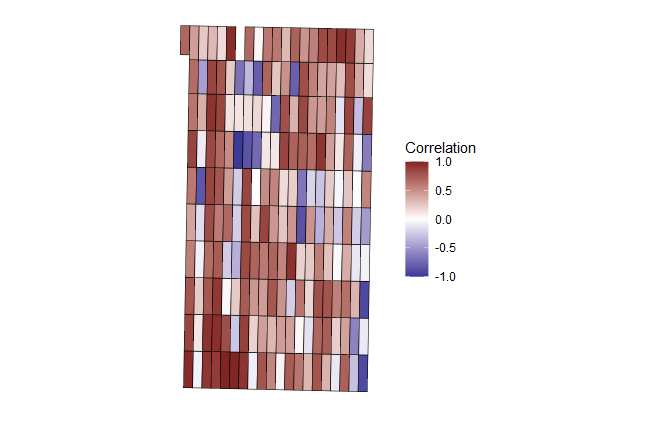
\includegraphics{../images/paper/corr-plot2.png}

}

\caption{\label{fig-redesign3}This plot directly states the relationship
(correlation) between the as-applied treatment information and crop
yield.}

\end{figure}

Next, we wanted to provide a more direct statement of the correlation
between input application rates and yield (Figure~\ref{fig-redesign3}),
as determination of this relationship through color blending may be
difficult and time-consuming for some users. Directing statign the
correlation uses another comparative layout: explicit encoding. Explicit
encoding is helpful as it displays the encoding of the relationship,
which spares the viewer of the effort to find it \citep{gleicher2011}.
We wanted to maintain some spatial information when presenting the
correlation, as field location may also play a role in this relationship
through variables like soil type. First, we used the as-applied
treatments as this is the true treatment amount applied to the field.
Second, to maintain spatial awareness, the correlation between the
as-applied and yield measurement \svp{was calculated} within each trial
plot (outlined by black boxes). A diverging color palette was used, as
correlation values have both magnitude and sign, using blue for
negatively correlated values and red for positively correlated values,
with a neutral color of white representing no correlation
\citep{macdonald_1999}. This is due to the common cultural association
of blues for negative numbers and red for positive numbers when used in
conjunction. The viewer now directly sees the relationship between the
variables while maintaining some spatial orientation through the trial
plots.

\begin{figure}

{\centering 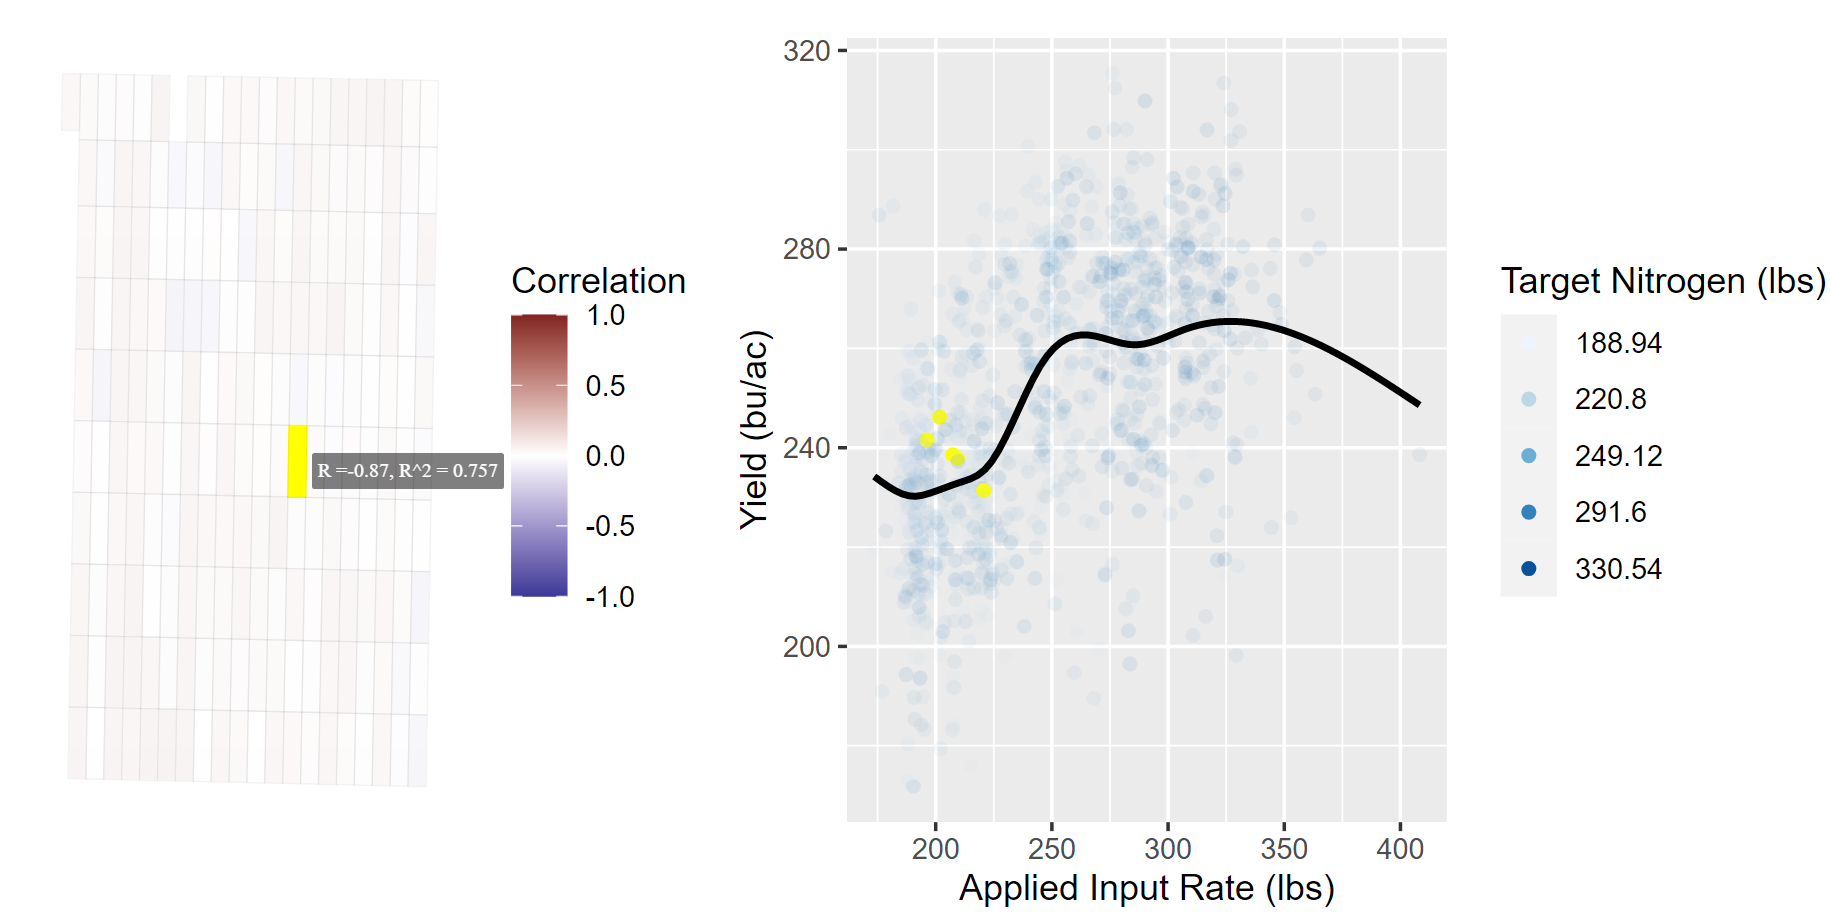
\includegraphics{../images/paper/corr-with-scat3.png}

}

\caption{\label{fig-redesign4}This figure overcomes the
decontextualization weakness of Figure 5 by juxtaposing the correlation
plot with a scatterplot of the values used in the correlation
calculations. They are connected using interactivity.}

\end{figure}

Unfortunately, while the relationship between the variables was directly
encoded, it can be complicated to connect the displayed relationship
back to the data \citep{gleicher2011}. Meaning, while the plot states
the correlation, it gives no additional information on the application
rate or yield. Hence we do not know what application rates are leading
to the higher yield values or how large the yield values are. A standard
practice to overcome this weakness is utilizing a hybrid comparative
layout \citep{lyi2021}. A scatterplot was juxtaposed to the correlation
plot (combining the layouts of juxtaposition and explicit encoding) to
add some context back. Interactivity connects the juxtaposed plots,
where hovering over a trial plot in the correlation map highlights the
corresponding data in the scatterplot used to perform the calculation
(Figure~\ref{fig-redesign4}). Hovering over a trial plot also inform the
user of the exact correlation (\(R\)) and also the coefficient of
determination (\(R^2\)). On the other side, if the user hovers over a
point on the scatterplot, the plot will display the point's target input
application, as applied input, and yield amount. It will then highlight
the corresponding trial plot and all other points on the scatterplot in
the same trial plot. Additionally, a trend line was added to the
scatterplot to display the overall trend of the data. While not
beneficial in static pdf reports, interactivity will be advantageous in
a future application designed to help farmers explore their data and
facilitate improved management decisions. In the scatterplot, the same
blue color palette, to represent the target rates, was used as in
Figure~\ref{fig-redesign2} to help users to connect those plots.

\hypertarget{discussion}{%
\section{Discussion}\label{discussion}}

While reviewing DIFM reports and journal articles produced through this
project, we found the regular use of sub-optimal plots to display the
relationship between crop target input application and crop yield.
Running themes found in these plots include data points overlapping and
the choice of an inappropriate color scheme. In redesigning these plots,
we used a superimposed comparative layout to limit the extent of the
comparative burden placed on the users. Figure~\ref{fig-redesign2} shows
our first proposed plot. This plot is an improvement due to the
nonoverlapping polygons made from the overlapping yield measurements, so
individual measurements are no longer obscured. Additionally, we
suggested a better color scheme (red-blue), as these colors do not
overlap and are more color-blind friendly. Blending the red and blue
color scales represents the relationship between the variables, where,
for example, the dark regions represent high target input application
and high yield. A drawback of this map is that areas of low target input
application/high yield and high target input application/low yield may
be hard to differentiate easily. Further, this design has difficulty
displaying the individual values of the variables. However, in viewing
the plot on a web page, we can use the \emph{leaflet} package in
\emph{R} to allow the user to display the maps individually or
superimposed.

Figure~\ref{fig-biv-map} introduces a bivariate color map to improve on
the drawback of the color-blended map. In this map, quantiles divided
each of the variables into three categories, where the crossing of the
categories resulted in nine groups, each assigned a unique color (lower
left). A benefit of the bivariate color map is its ability to easily
denote the values along the diagonal of the color legend or those that
display a positive linear relationship. Moreover, the low target input
application/high yield and high target input application/low yield
categories are easily recognized. However, a drawback of this method is
that individual values are not distinguishable due to the categories.
Further, individual information about each variable can not be
separated, like in the color-blended map. In addition, due to trying to
work within memory limits, the categories of each variable may cover a
wide range of values and do not give detailed information
\citep{roth-2017}. Technically, the number of colors used is more than
the recommendation of seven, but only five are of real interest
(diagonal and the other two corners). A scatterplot of the applied input
data versus the crop yield was juxtaposed with the color scheme as the
background (Figure~\ref{fig-biv-scat}) to gain additional information.
The scatterplot was to add some context on what the data looks like
within each category.

Finally, we developed a plot that directly states the relationship
between input application and crop yield using the explicit encoding
comparative layout. This plot (Figure~\ref{fig-redesign3}) displays the
calculated correlation within each trial plot, as spatial location plays
a vital role in this relationship. Spatial location is significant due
to spatially varying variables like soil type and precipitation on a
field. Now the users no longer have to infer the correlation themselves.
To counteract the negative qualities of explicitly encoded graphs (not
displaying the data), a scatterplot of the actual data used in the
calculations was added to the right-hand side. In
Figure~\ref{fig-redesign4}, the two plots are linked, so the data used
to calculate the correlation in a trial plot on the left is highlighted
in the scatterplot on the right. Hence, this plot directly states the
relationship while also linking to the data. Unfortunately, this version
is not compatible with static pdf reports.

The suggested improvements of the original plots follow what is
currently known about effective data visualization to help users
understand the desired information by avoiding overlapping data points
and choosing more effective colors. The next step in this process is to
obtain feedback from those using these plots (farmers, researchers, crop
consultants) to see which of the suggested plots is preferred and to
tweak any of the designs if necessary. In the future, these specific
plots will be used in DIFM reports and publications, while the
suggestions made during the creation of these plots can be used in other
applications for displaying two variables in a spatial domain in the
agricultural domain.


\renewcommand\refname{References}
  \bibliography{bibliography.bib}


\end{document}
